%!TEX TS-program = xelatex
%!TEX encoding = UTF-8 unicode
\documentclass[12pt]{article}

\usepackage[svgnames]{xcolor}
\usepackage{sslides}
\usepackage{graphicx}
\usepackage{verbatim}
\usepackage{textcomp}
\usepackage{mathptmx} % Times
\usepackage[scaled=.90]{helvet}
\usepackage{courier}
\usepackage{fontspec}
\usepackage{tikz}
\usepackage{framed}
\setmainfont[Mapping=tex-text,Ligatures={Common,Rare,Discretionary}]{Linux Libertine O}
\newfontfamily\quotefont[Mapping=tex-text,Ligatures={Common,Rare,Discretionary}]{Linux Libertine O}

\def\nameTitle{Yoan Blanc}
\def\emailTitle{\texttt{yoan.blanc@epfl.ch}}
\def\affiliationTitle{IN, EPFL}
\def\placeAndDayTitle{December 20\textsuperscript{th}, 2012}

\def\presentationTitle{Fish-eye transformation with bilinear interpolation}
\def\presentationSubTitle{CS-425 Program parallelization on PC clusters}

\definecolor{Emph}{rgb}{0.8,0.2,0.2}  %softer red for display
\definecolor{Title}{rgb}{0.2,0.2,0.8}  %softer blue for display

% http://tex.stackexchange.com/questions/16964/block-quote-with-big-quotation-marks
% Make commands for the quotes
\newcommand*{\openquote}{\tikz[remember picture,overlay,xshift=-15pt,yshift=-10pt]
\node (OQ) {\quotefont\fontsize{60}{60}\selectfont``};\kern0pt}
\newcommand*{\closequote}{\tikz[remember picture,overlay,xshift=15pt,yshift=10pt]
\node (CQ) {\quotefont\fontsize{60}{60}\selectfont''};}
% select a colour for the shading
\definecolor{shadecolor}{named}{Azure}
% wrap everything in its own environment
\newenvironment{shadequote}%
{\begin{snugshade}\begin{quote}\openquote}
{\hfill\closequote\end{quote}\end{snugshade}}


\begin{document}


%% add entry for Titleslide
\addcontentsline{toc}{subsection}{\protect\numberline{\thesection}Title slide}%

%% Title slide

\vspace{3cm}

\raggedright \textcolor{Title}{\LARGE\bf \presentationTitle} \\[3mm]
\textcolor{Title}{\presentationSubTitle}

\vspace{2cm}

\raggedright {\bf \nameTitle} \\[2mm]
{\small\affiliationTitle}
\vspace{2cm}

\raggedright {\small \placeAndDayTitle}

\thispagestyle{empty}

\section{Fisheye 101}
\begin{center}
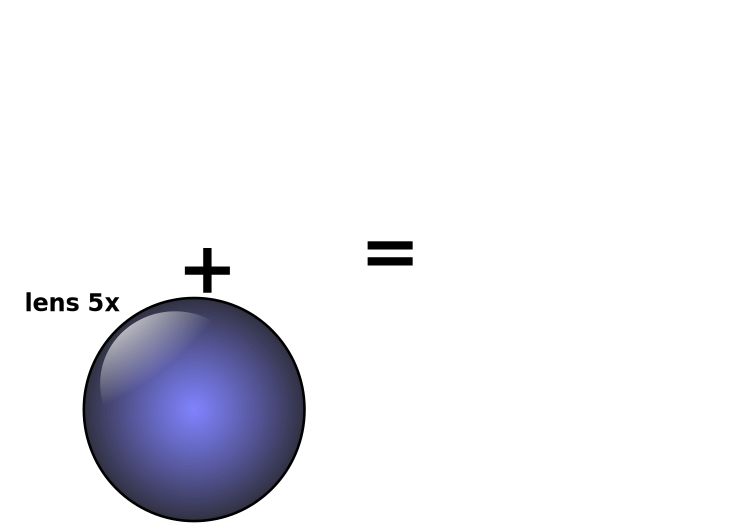
\includegraphics[width=.8\textwidth]{../figures/101.png}
\end{center}

\section{In a nutshell}
\begin{center}
\includegraphics{../figures/serial.png}
\end{center}

\begin{comment}
\section{}
\vspace{3cm}
\begin{shadequote}
    \LARGE \emph{FIRST OPTIMIZE ON ONE CORE, THEN PARALLELIZE (the right
    algorithm)} \\
    \large ---Vincent Keller
\end{shadequote}
\end{comment}

\section{Serial versions}

\begin{itemize}
    \item \textbf{compute} only $\frac{1}{8}$ of the lens
    \item \textbf{I/O:} uses memory mapping (\texttt{mmap} on Linux)
\end{itemize}

\begin{center}
    \begin{minipage}[b]{0.45\linewidth}
        \includegraphics[width=\textwidth]{../../plots/areatime_total_linear.png}
    \end{minipage}
    \begin{minipage}[b]{0.45\linewidth}
        \includegraphics[width=\textwidth]{../../plots/areatime_total_log.png}
    \end{minipage}
\end{center}

\small Running on BC 07 machines.

\section{Time breakdown}

\vspace{3cm}
\begin{center}
\begin{tabular}{ l | l | c | c  || c}
    Machine & Algorithm & I/O & Computation & Total \\
    \noalign{\medskip}
    \hline \hline
    \noalign{\medskip}
    GNU/Linux (BC07) & Serial 5 & 0.2 & 9.2 & 9.4 \\
    \noalign{\medskip}
    \hline
    \noalign{\medskip}
    Windows (INF2) & Serial 4 & 70 & 18 & 88 \\
\end{tabular}
\end{center}

\vspace{3cm}
\small Picture used: 8000x8000 24bits BMP, \url{http://flic.kr/p/binsBK}

\section{MPI 0}

Distributed lens \textbf{computation}.

\begin{center}
\includegraphics[width=.8\textwidth]{../figures/mpi0.png}
\end{center}

\section{MPI 1}

Distributed lens \textbf{application}

\begin{center}
\includegraphics[width=.8\textwidth]{../figures/mpi1.png}
\end{center}

\section{Computation/communication}

MPI, on INF2 machines:
\begin{itemize}
    \item Lens size: $3600^2 \cdot 2 = 24 MB$
    \item Picture size:  $7200^2 \cdot 3 = 148 MB$
    \item Computational time: $18 sec$
    \item Total data: $24 + 148 = 172 MB$
    \item Communication time: $\frac{172}{9.7} = 17.7 sec$
\end{itemize}

$$Ratio = \frac{18}{17.7} \simeq 1$$

\small Measured bandwidth in INF3: $9.7MB/s$, latency: $5.75ms$

\section{MPI}

\begin{itemize}
    \item \textbf{MPI 0} distributed lens computation while loading.
    \item \textbf{MPI 1} local lens comput. and distributed application.
\end{itemize}

\begin{center}
    \begin{minipage}[b]{0.45\linewidth}
        \includegraphics[width=\textwidth]{../../plots/areatime_total_linear_mpi.png}
    \end{minipage}
    \begin{minipage}[b]{0.45\linewidth}
        \includegraphics[width=\textwidth]{../../plots/mpi_speedup_total_8000_no_ideal.png}
    \end{minipage}
\end{center}

\small Running on INF 2 machines.

\section{Amdahl's law}

Shared memory (OpenMP), on BC machines:

$$f = \frac{0.2}{9.4} = 0.02$$
$$S_p \le \frac{1}{f + \frac{1 - f}{p}} = \frac{1}{0.02 + \frac{0.98}{p}}$$

\section{OpenMP}

\begin{itemize}
    \item \textbf{OpenMP 0} parallel loading and lens computation
    \item \textbf{OpenMP 1} parallel lens comput. and application
\end{itemize}

\begin{center}
    \begin{minipage}[b]{0.45\linewidth}
        \includegraphics[width=\textwidth]{../../plots/areatime_total_linear_omp.png}
    \end{minipage}
    \begin{minipage}[b]{0.45\linewidth}
        \includegraphics[width=\textwidth]{../../plots/omp_speedup_total_8000.png}
    \end{minipage}
\end{center}

\small Running on BC 07 machines.

\section{Conclusion \& Future plans}

\begin{itemize}
    \item \textbf{I/O} is hard.
    \item Investigate \textbf{MPI\_File}.
    \item MPI version able to split the picture into 8 (or more) slices.
\end{itemize}

\section{Fin}
\vspace{4cm}
\begin{center}
\emph{Danke sehr, Merci, Grazie…}

\textasteriskcentered \textasteriskcentered \textasteriskcentered

\emph{…and Merry Holidays!}
\end{center}

\end{document}
